% CVPR 2025 Paper Template; see https://github.com/cvpr-org/author-kit

\documentclass[10pt,twocolumn,letterpaper]{article}

%%%%%%%%% PAPER TYPE  - PLEASE UPDATE FOR FINAL VERSION
% \usepackage{cvpr}              % To produce the CAMERA-READY version
\usepackage[review]{cvpr}      % To produce the REVIEW version
% \usepackage[pagenumbers]{cvpr} % To force page numbers, e.g. for an arXiv version

% Import additional packages in the preamble file, before hyperref
%
% --- inline annotations
%
\newcommand{\red}[1]{{\color{red}#1}}
\newcommand{\todo}[1]{{\color{red}#1}}
\newcommand{\TODO}[1]{\textbf{\color{red}[TODO: #1]}}
% --- disable by uncommenting
% \renewcommand{\TODO}[1]{}
% \renewcommand{\todo}[1]{#1}

\usepackage{float}

\usepackage{tikz} % draw figures
\usepackage{siunitx} % units and maths
%\usepackage{minted} % code highlighting
\usepackage{makecell} % break line in table cell


% It is strongly recommended to use hyperref, especially for the review version.
% hyperref with option pagebackref eases the reviewers' job.
% Please disable hyperref *only* if you encounter grave issues,
% e.g. with the file validation for the camera-ready version.
%
% If you comment hyperref and then uncomment it, you should delete *.aux before re-running LaTeX.
% (Or just hit 'q' on the first LaTeX run, let it finish, and you should be clear).
\definecolor{cvprblue}{rgb}{0.21,0.49,0.74}
\usepackage[pagebackref,breaklinks,colorlinks,allcolors=cvprblue]{hyperref}

%%%%%%%%% PAPER ID  - PLEASE UPDATE
\def\paperID{*****} % *** Enter the Paper ID here
\def\confName{CVPR}
\def\confYear{2025}

%%%%%%%%% TITLE - PLEASE UPDATE
\title{Unlock and Compare the most Accurate Publicly Available AI Models for your Tasks}

%%%%%%%%% AUTHORS - PLEASE UPDATE
\author{Antoine Meyer\\
National Institute of Standards and Technology\\
100 Bureau Dr, Gaithersburg, MD 20899\\
{\tt\small https://orcid.org/0009-0007-5693-5760}
% For a paper whose authors are all at the same institution,
% omit the following lines up until the closing ``}''.
% Additional authors and addresses can be added with ``\and'',
% just like the second author.
% To save space, use either the email address or home page, not both
\and
Mylene Simon\\
{\tt\small mylene.simon@nist.gov}
\and
Peter Bajcsy
{\tt\small peter.bajcsy@nist.gov}
{\tt\small https://orcid.org/0000-0002-6968-2615}
}

\begin{document}
\maketitle

\cite{Authors14}, \cite{Authors14b}


\begin{abstract}
This paper aims to present the work carried out to (1) increase the number of
Artificial Intelligence (AI) models usable in a scientific workflow engine
called Web Image Processing Pipeline (WIPP), (2) document the AI models used,
and (3) compare results of executing different AI models on the same dataset in
order to select the best.
\TODO\

\end{abstract}
\section{Introduction}
\label{sec:intro}

With the relentless development of Artificial Intelligence (AI), new
architectures and new ways of analyzing texts and images are leading to many new
models. This enthusiasm enables us to meet a wide range of needs but analyzing
all these tools and choosing the right AI model to best solve your specific
problem is becoming less and less straightforward.

\Gls{latex}

Building a model from scratch for a specific application is time-consuming and
tedious. Numerous public repositories of AI models exist, avoiding this
preliminary work and allowing you to concentrate on use (inference) and/or
adjustments (finetuning). It is therefore vital to be able to select the most
accurate pre-trained model from those available, if possible, as automatically
as possible.

\cite{Authors14}, \cite{Authors14b}


This motivation of reusing pre-trained models from public repositories poses
three major challenges: (1) there is no standard API to access public
repositories with trained AI models, (2) there is insufficient metadata about
trained AI models in public repositories to match them to applications and to
run them, and (3) there is no way of automatically assessing the accuracy of AI
models.

The first challenge is partly facilitated by the Application Programming
Interface (API) offered by certain platforms, such as Transformers for Hugging
Face. However, this is not the case for all AI model repositories and Web Image
Processing Pipeline (WIPP) has yet to implement these APIs. The second challenge
also has a start of a solution in the shape of the Model Card concept. However,
information is often scanty if not completely absent and is not automated.
Finally, the third challenge requires special development to enable calculation
of one way to evaluate models results accuracy as the Dice-Sørensen coefficient.

\section{Methods}
\label{sec:methods}

Web Image Processing Pipeline (WIPP) is a scientific workflow engine,
illustrated as shown in figure 1. This tool enables all kinds of image
visualization and analysis. The workflow concept enables a sequence of plugins,
a piece of code put in the form of a container, allowing all kinds of analysis
or modification.

\begin{figure}[H]
  \centering
  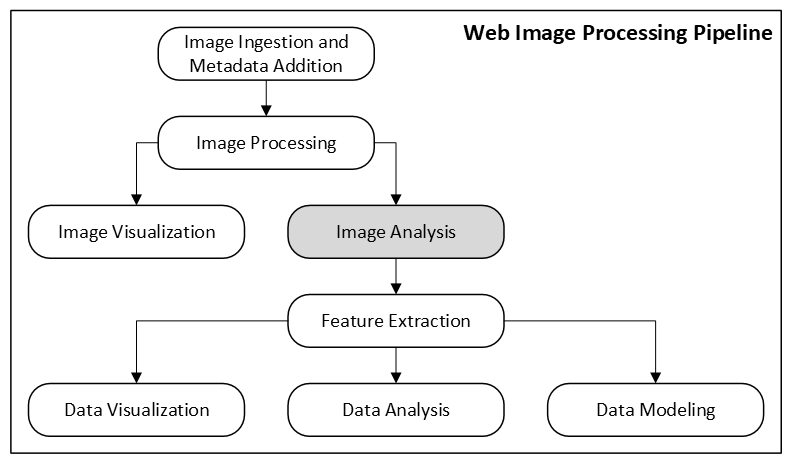
\includegraphics[width=0.8\linewidth]{png/1_wipp.png}
  \caption{Web Image Processing Pipeline}
  \label{fig:1wipp}
\end{figure}

Thanks to a plugin you can, for example, load an AI hosted in WIPP, specify an
image collection and perform the inference of this AI on the selected images.
The result will be a new collection of images modified by the AI, for example
with a label after inference of a classification model.

\subsection{Access public repositories via WIPP}

We have developed new inference plugins, see figure 2, to enable access to AI
models available on different public repositories.
\TODO ADD SAM2, ADD CELLPOSE here

\begin{figure}[H]
  \centering
  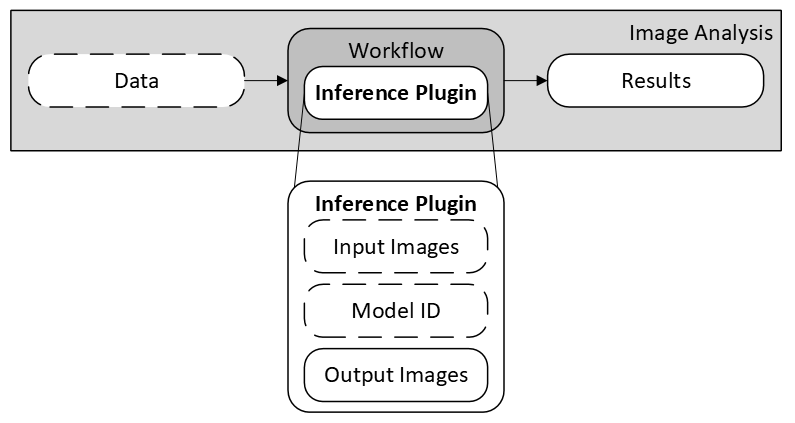
\includegraphics[width=0.8\linewidth]{png/2_inference_plugin.png}
  \caption{Inference Plugin}
  \label{fig:2inference}
\end{figure}

This was achieved by developing general-purpose code using the Application
Programming Interfaces (APIs) of the various platforms: Transformers for Hugging
Face and the BioImage.IO API. This enabled us to increase the number of
Artificial Intelligence (AI) models usable in WIPP thanks to containerized
software.

\subsection{Document AI models}

We have introduced AI model card entries that are necessary for matching tasks
with AI models. This information will also be needed as runtime parameters.
Figure 3, training an AI in WIPP automatically generates its documentation
(model card).

\begin{figure}[H]
  \centering
  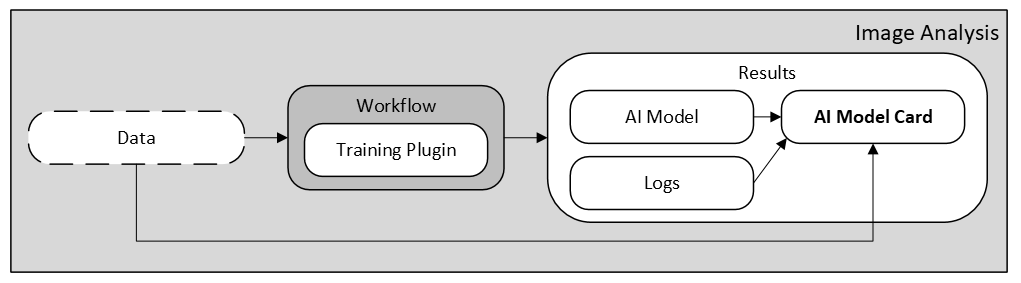
\includegraphics[width=0.8\linewidth]{png/3_ai_model_card.png}
  \caption{AI Model Card}
  \label{fig:3aimodelcard}
\end{figure}

This was achieved by developing code to retrieve information about the AI model
throughout the pipeline: name, creation date, data used for training, number of
iterations, training time, and more.

\subsection{Compute accuracy}

We have developed a new plugin, see figure 4, to compute the Dice-Sørensen
coefficient. It is a statistic used to gauge the similarity of two samples, in
our case images.

\begin{figure}[H]
  \centering
  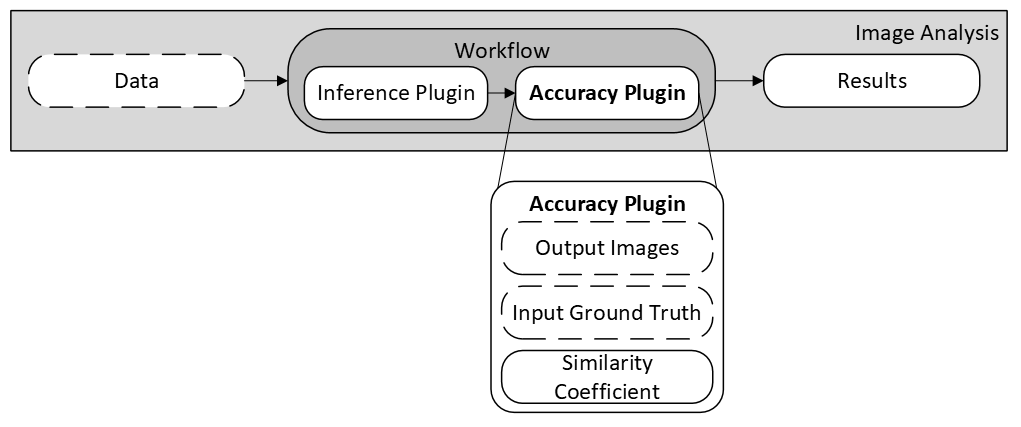
\includegraphics[width=0.8\linewidth]{png/4_accuracy.png}
  \caption{Accuracy Plugin}
  \label{fig:4accuracy}
\end{figure}

This was achieved by implementing the Sørensen's formula into a containerized
software (plugin). This makes it now possible to sequence model inference (a
model created within WIPP, as in workflow 1, or a model from a repository such
as Hugging Face, as in workflow 2) and evaluate the accuracy of the result
provided, by comparing it with ground truth data.

\section{Results}
\label{sec:results}

Access new repositories give access to a lot of new models usable in Web Image
Processing Pipeline (WIPP). It also saves hours of computational time and
resources, as well as improves reusability of pre-trained AI models.

In the context of Image Analysis in WIPP, we are looking to use Mask
Generation Models.

\begin{table}[H]
\centering
\caption{\label{tab:number_of_newly_available_models}%
  Number of newly available Mask Generation models
}
\begin{tabular}{lc}
  \toprule
  Repository & Mask Generation Model(s) \\
  \midrule
  WIPP & 1 \\
  Hugging Face & 176 \\
  BioImage.IO & 32 \\
  Cellpose & 21 \\
  SAM2 & 8 \\
  \bottomrule
\end{tabular}
\end{table}

The level of documentation varies greatly from model to model. We have set up an
automatic documentation system for models trained within WIPP.

Finally to avoid lower confidence in external models, we have developed a way of
evaluating the results and therefore the relevance of the models tested, in
order to select and retain only those that deliver the best results.

\subsection{WIPP compute with 3D-RPE data}

Masks used are here
https://wipp-dev.nist.gov/images-collection/671abb516103440e64a77397 and images
used are here
/mnt/isgnas/project/csmet/bio/Proj-028-RPE-Measurements/sample\_data\_2024-10-24.
The WIPP server specifications are \TODO\

\begin{table}[H]
\tiny
\centering
\caption{\label{tab:comparative_results_for_different_models}%
  Comparative models results run in WIPP
}
\begin{tabular}{llcc}
  \toprule
  Repository & Model Name & Inference Time per Image (s) & Accuracy (\%) \\
  \midrule
  WIPP & WIPP UNet CNN 1.0.0 & \TODO\ &  \\
  Hugging Face & facebook/sam-vit-huge & 7.04 & $\SI{40.62}{\percent} \pm \SI{34.99}{\percent}$ \\
               & Zigeng/SlimSAM-uniform-50 & 939s/162 images = 5.79 & $\SI{25.05}{\percent} \pm \SI{22.02}{\percent}$ \\
               & jadechoghari/robustsam-vit-large & 6.76 & $\SI{38.19}{\percent} \pm \SI{35.67}{\percent}$ \\
  BioImage.IO & 10.5281/zenodo.5869899 & ISSUE WITH DOCKER &  \\
              & 10.5281/zenodo.5764892 &  &  \\
  Cellpose & cyto3 & \TODO\ &  \\
           & nuclei & \TODO\ &  \\
  SAM2 & facebook/sam2.1-hiera-large & 2.12 & $\SI{38.16}{\percent} \pm \SI{35.02}{\percent}$ \\
       & facebook/sam2-hiera-small & \TODO\ &  \\
  \bottomrule
\end{tabular}
\end{table}

\subsection{Local compute with 3D-RPE data}

Data used are the same from above. The local computer specifications are one GPU
Quadro RTX 4000 with CUDA version 12.7 and Memory 8192 MiB.

\begin{table}[H]
\tiny
\centering
\caption{\label{tab:comparative_results_for_different_models}%
Comparative models results run in local
}
\begin{tabular}{llcc}
  \toprule
  Repository & Model Name & Inference Time per Image (s) & Accuracy (\%) \\
  \midrule
  Hugging Face & facebook/sam-vit-huge & \TODO\ &  \\
               & Zigeng/SlimSAM-uniform-50 & \TODO\ &  \\
               & jadechoghari/robustsam-vit-large & \TODO\  &  \\
  BioImage.IO & 10.5281/zenodo.5869899 & \TODO\ &  \\
              & 10.5281/zenodo.5764892 & \TODO\  &  \\
  Cellpose & cyto3 & \TODO\ &  \\
           & nuclei & \TODO\  &  \\
  \bottomrule
\end{tabular}
\end{table}

\subsection{Local compute with RPEimplants data}

Data used are from this link https://isg.nist.gov/deepzoomweb/data/RPEimplants.
They contains images of 2D Measurement of Retinal Pigment Epithelium Function
Using Quantitative Bright-Field Microscopy. Local computer specifications are
the same as above.

\begin{table}[H]
\tiny
\centering
\begin{tabular}{llcc}
  \toprule
  Repository & Model Name & Inf. Time per Image (s) & Accuracy (\%) \\
  \midrule
  Hugging Face & facebook/sam-vit-huge & 4.16 & $\SI{85.87}{\percent} \pm \SI{3.98}{\percent}$ \\
                & Zigeng/SlimSAM-uniform-50 & 2.81 & $\SI{79.78}{\percent} \pm \SI{5.31}{\percent}$ \\
                & jadechoghari/robustsam-vit-large & \TODO\ &  \\
  BioImage.IO & 10.5281/zenodo.5869899 & 0.31 & $\SI{89.30}{\percent} \pm \SI{0.84}{\percent}$ \\
              & 10.5281/zenodo.5764892 & 0.38 & $\SI{10.44}{\percent} \pm \SI{3.20}{\percent}$ \\
  Cellpose & cyto3 & \TODO\ &  \\
            & nuclei & \TODO\  &  \\
  \bottomrule
\end{tabular}
\end{table}

---

Even if the results may not be perfect, this method allows you to quickly try
out a new model at reduced cost. It is also easy to change dataset. We can then
take a promising model and improve it by finetuning it. We hope to improve the
speed of data analysis within WIPP and enable better overall results.

\section{Discussion}
\label{sec:discussion}

\TODO\



{
    \small
    \bibliographystyle{ieeenat_fullname}
    \bibliography{main}
}

% WARNING: do not forget to delete the supplementary pages from your submission
% \input{sec/X_suppl}

\end{document}
